\chapter{Model architecture and processes}
\label{ch:design}

In this chapter, both the architecture and the training and inference mechanisms of a concrete system are described. We begin by delimiting the scope of the system develop for this project. Next, we present the overall architecture of the system, followed by specific sections devoted to the different parts of the system: encoder, decoder. Finally, we describe the methods used to train and evaluate the system.

\section{Scope}\label{sec:scope}

Before diving into the design of the system developed for this project, it seems convenient to delimit the scope of it as well as justify the design decisions taken. In particular, we have to decide on three main separated aspects:

\begin{enumerate}
\item To begin with, we should decide on the kind of architecture to design our system, which can further be divided into various finer details, like deciding the concrete models to use for each component of the architecture, whether to use transfer learning, and whether to use ensemble methods, among others.
\item Another decision of high importance if the dataset to use in order to train and evaluate our system. As a secondary decision, we should also decide which metrics to use for evaluating it.
\item Finally, we should decide on the specific experiments, which in turn will involve deciding on various hyper-parameters and configuration options that may be available in our model.
\end{enumerate}

Deciding on those three aspects should be conditioned by a combination of factors, from research considerations to hardware requirements and time constraints. This chapter will briefly discuss on these aspects, and then we will conclude with the final decisions that define the scope of the system to be developed as part of this project.

\subsection{Research considerations}

As we have seen in our review of the state of the art (\cref{ch:state_of_the_art}), image captioning is a thrilling field of research that have seen tremendous advances in recent years, specially since neural networks and deep learning were applied to it. From the first neural model proposed by \citet{Kiros2014_LBL}, a myriad of different neural models have been proposed, usually combining a visual encoder and a text decoder. Although there are some exceptions, the majority of the models proposed so far use some form of Convolutional Neural Network (CNN) for the encoder, and some form of Recurrent Neural Network (RNN) for the decoder. Some models  also use CNN for the decoder, and a few recent models include Generative Adversarial Networks (GAN) to achieve more varied and expressive captions. Most of models proposed use some form of supervised learning, typically back-propagation, but there is a growing number of models that include reinforcement learning, and there have been some recent attempts to use also semi-supervised learning, and even unsupervised learning. 

Summing up, there are many options to choose from in order to develop our own image captioning system. If we look at the results obtained from these models in benchmark datasets, we can see various patterns and trends.

\begin{itemize}
\item First, end-to-end approaches based on the encoder-decoder framework prevail over compositional architectures.
\item Second, attention mechanisms have flourished and are a key component included in the vast majority of models, although they can adopt different forms.
\item Third, the addition of reinforcement learning is gaining a lot of momentum as a means to improve the quality of generated captions when considering language quality metrics such as CIDEr.
\item Fourth, models tend to increase in complexity by stacking more layers and including additional methods and forms of learning. Another aspect of this trend is the use of ensemble methods that combine various models together to produce the final result.
\end{itemize}

Besides the aforementioned trends and patterns, the study of the published research relative to image captioning reveals a 
high degree of alignment between this research and the more general research sequence-to-sequence (\textit{seq2seq}) learning and sequence translation problems. Therefore, it would be interesting to study current trends in \textit{seq2seq} research to anticipate the next advances in image captioning.

Indeed, neural image captioning systems adopted the encoder-decoder architecture used in sequence translation, with the particularity of using CNN for the encoder, but the decoder is a RNN as those used in seq2seq problems. Next, ResNet and Attention make its appearance, and rapidly gained popularity, both in seq2seq learning and image captioning.

Attention-based networks are increasingly used by the big players in the IT world, including Google and Facebook. The main reason from this shift from simple RNN to attention-based architectures is because the former require more resources to train and run than the latter. Therefore, we deem attention as a key ingredient to include in our own system.

\subsection{Hardware requirements and time constraints}

Although for some projects hardware and time may appear as two separate aspects to factor in, they are closely related when we are dealing with deep learning. That is because due to the vast size of some datasets, training some systems may require either fabulous hardware resources or incredibly long periods, and even a combination of both.

For this project we have to deal with a combination of both little time and limited hardware resources, so we have to limit the scope of our project to something manageable.

At the beginning of this project, we had at our disposal a computer equipped with an NVIDIA GTX 1070 GPU supporting CUDA, which is a must-have for any deep learning project beyond toy examples.

After doing some preliminary experiments we realized that with the hardware at hand, it was going to be unfeasible to work with current state of the art benchmark datasets such as MS COCO (not to mention the Conceptual Captions dataset, recently released by Google). Furthermore, we got serious problems when using the computer in interactive mode whilst training a deep learning model. 

One option was to conduct our experiments on a smaller, dataset such as the Flickr8K or perhaps the Flickr30K dataset, but there are quite outdated nowadays. Therefore, in order to work with bigger datasets I decided to invest in a new, more powerful GPU, and so I bought an NVIDIA GTX 20180 Ti. I got this GPU installed in the same computer, alongside the GTX 1070. As a result of the new configuration, the training times reduced considerably, and it become feasible to use the computer whilst training a model on the COCO dataset.

The most relevant specifications of the final hardware used to conduct the experiments as as follows:

\begin{itemize}
\item CPU: Intel Core i7-4790K (4 cores, 8 threads clocked @ 4 GHz)
\item RAM: 16GB DIMM DDR3 2400 (clocked @ 1333 MHz)
\item Storage: 2 x SSD Samsung 850 Evo 250GB
\item GPU-0: NVIDIA GTX 1070, 6GB RAM
\item GPU-1: NVIDIA RTX 2080 Ti, 11GB RAM
\end{itemize}

Note the two GPUs included in the system. The GTX 1070 is used as the rendering unit, for interactive tasks, while the RTX 2080 Ti is used as the main CUDA platform to carry on the data intensive tasks required to train and evaluate our model on big datsets. With that hardware, we deem it possible to train models one the full COCO dataset in less than a week, depending on the concrete architecture of the net and different hyper parameters on the net, as well as some restrictions imposed on the training data, such as the size of the vocabulary, or the maximum caption length allowed.

\subsection{Software requirements}

With respect to the software requirements, from the very beginning of the project, it was decided to met two kind of requirements:
\begin{itemize}
    \item Using a language we are familiar with
    \item Using a popular framework with a big community 
\end{itemize}

The combination of the two requisites above led us to choose Python as the development language, and Keras with Tensorflow backend as the computational framework. 

However, in the end we decided to take a little risk by using an alpha version of the Keras-Tensorflow stack that has been released recently, \textbf{Tensorflow 2.0.0-alpha}.

\subsection{Summing up}

The study of published research resulted in the selection of an \textbf{encoder-decoder architecture with a soft attention mechanism} based on the model proposed by \citet{Xu2015}. 

However, there are so many options to choose from for the different components of our system, that we should limit those options to a few options.
\begin{itemize}
    \item \textbf{Encoder}: we aim at trying at least two different encoders, like the Inception-V3 network, and the NASNet.
    \item \textbf{Decoder}: for this component, the idea is to try both GRU and LSTM units. 
    \item \textbf{Attention} mechanism: we aim at trying the soft attention mechanism, which is easier to implement
\end{itemize}

Finally, if there is enough time we may try different hyper-parameters, such as the number of hidden units or units in the embedding layer. Other options to play with are the size of the vocabulary, but that is difficult to estimate at this stage of the project.

\section{Overall architecture}

As we have discussed in previous section \cref{sec:scope}, we have decided to develop an end-to-end deep learning solution to the image captioning problem based on an \textbf{encoder-decoder architecture} with an \textbf{attention mechanism}. This is so far the most common architecture used by state of the art systems, as we have seen in our review of the field (\cref{ch:state_of_the_art}.) More specifically, our system will consist of the following components:

\begin{itemize}
    \item Encoder made of a Convolutional Neural Network (CNN)
    \item Decoder made of a Recurrent Neural Network (RNN)
    \item Soft Attention mechanism
\end{itemize}


\begin{figure}[hpt]
	\centering
	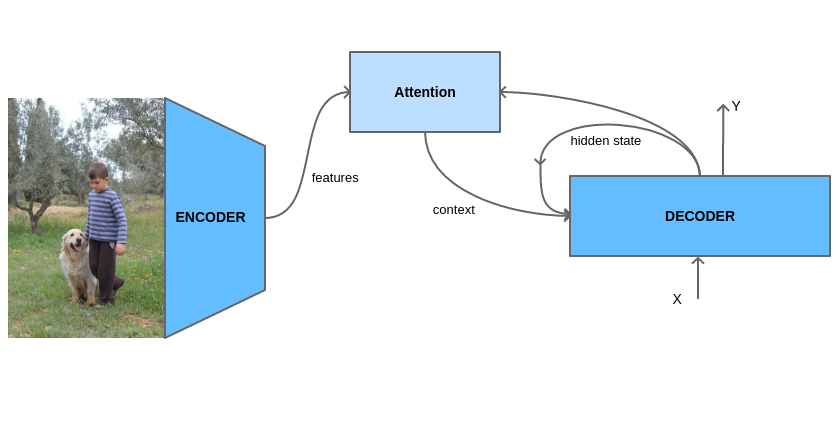
\includegraphics[scale=0.5]{images/ch4/overview.png}
	\caption{Overall system architecture: encoder-decoder with soft attention}
	\label{fig:overview}
\end{figure}

The general architecture of the system is depicted in \cref{fig:overall-architecture}. To the left of the figure, there is the encoder, which takes an image as input and extracts a feature map. To the right, the decoder has to produce a caption for the input image, using information from its input, its hidden state, as well as the context information received from the attention mechanism. The attention mechanism lies in between the encoder and the decoder. It is responsible of deciding on which parts of the image (on which features) to focus at each time step while. The attention mechanism take the image features and the hidden state of the decoder as inputs, and generates a context vector, which consists of the features weighted according to some learned weights, which represent the relevance given to each feature at a given moment.

Whilst the encoder generates the features in a single forward step, the decoder has to generate a caption word by word, one word at a time. To generate the next word it uses the information from past states, the current input (the last generated word), and the context information. The process of generating a caption as well as the training procedure will be describe later in this chapter.

A more detailed view of the architecture is provided in \cref{fig:overall-architecture}, showing the main layers used in the different components of the system. 
\begin{itemize}
    \item The encoder consists of a CNN module pretrained on the ImageNet dataset. We take the output from the last convolutional layer, and pass it through a dense, fully connected layer to flatten it before passing it to the attention module. 
    \item The decoder consists of an embedding layer that converts input tokens into embedding vectors, a recurrent layer, which may be made of either GRU or LSTM units, and two stacked fully connected layer that produce the final output. The input is a concatenation of the external input and the context vector from the attention mechanism.
    \item The attention mechanism actually consists of two fully connected layers, although they are not showed in the picture. It takes the flattenned features from the encoder as input, the hidden estates from the decoder, computes attention weights and produces a context vector as output.
\end{itemize}


\begin{figure}[hpt]
	\centering
	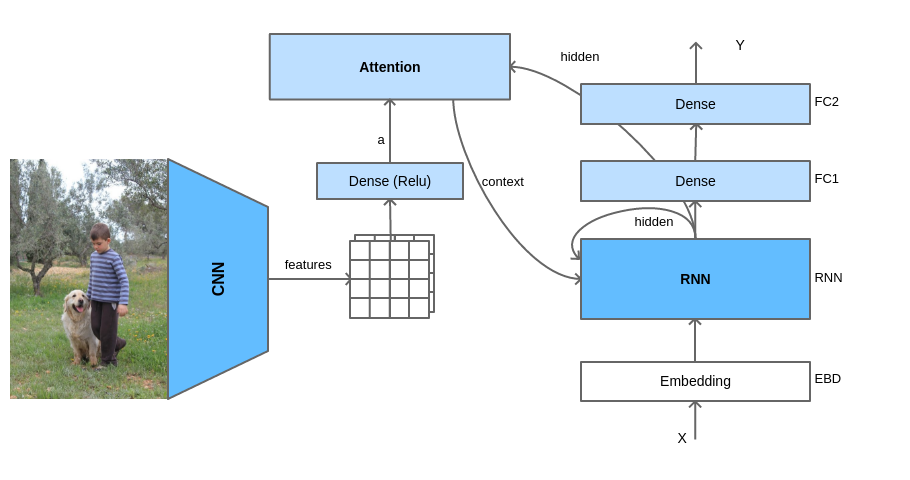
\includegraphics[scale=0.5]{images/ch4/overall-architecture.png}
	\caption{Overall system architecture: encoder-decoder with soft attention}
	\label{fig:overall-architecture}
\end{figure}


The following sections will describe each component of the network architecture in detail.

\section{Encoder}

The encoder consists of a \textbf{CNN} module \textit{pretrained} on the ImageNet dataset. Several options are available for this model. We have included some of the most popular convnets, including VGG-16\citep{Simonyan2015},Inception-V3\citep{Szegedy2016}, ResNet50\citep{He2016resnet}, and Xception \citep{Chollet2017}. We also tried to use the NASNet \citep{Zoph2018} large model, but it was impossible due to memory limitations\footnote{For a detailed description of how ConvNets work please check \cref{sec:cnn}. For a review of the most popular ConvNets, including some of the ones cited above, please see \cref{subsubsec:modern_cnn}.}.

As an example, let us assume we are using Inception-V3 for the CNN module. The architecture of this network is shown in \cref{fig:inceptionv3}.

\begin{figure}[hpt]
	\centering
	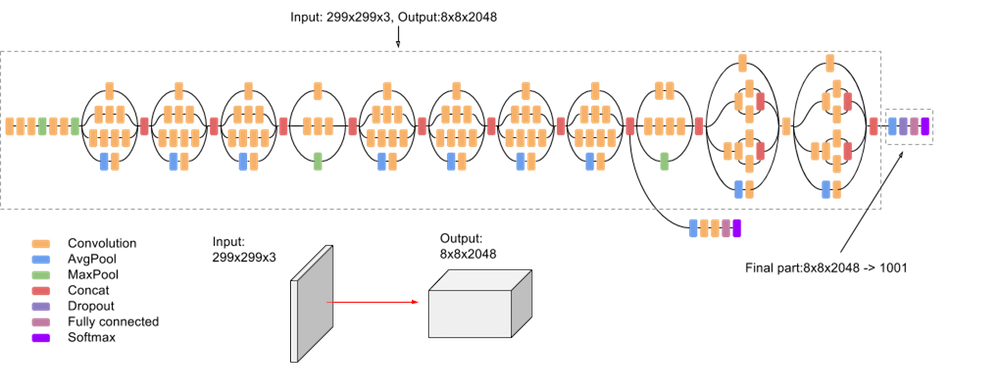
\includegraphics[scale=0.5]{images/ch4/inceptionv3.png}
	\caption{Overview of the Inception v3 network architecture. Source \href{https://cloud.google.com/tpu/docs/inception-v3-advanced}{Google's Advanced Guide to Inception v3 on Cloud TPU}}
	\label{fig:inceptionv3}
\end{figure}

This network receives an image represented by a 3D tensor with shape $(229, 229, 3)$, and generates an output consisting of 1001 logits, corresponding to the 1000 classification categories in the ImageNet dataset, plus an additional output to denote \textit{other} things not included in the labeled categories. However, we are interested in the last convolutional layer, just before entering the fully connected block. The output of a convolutional layer is a feature map organized as a grid of image patches and a number of features per image patch --the depth, or number of channels (see \cref{subsec:conv_layers}). As shown in \cref{fig:inceptionv3}, the output of the Inception-v3 network's last convolutional layer consists of $8 \times 8 \times 2048$ features, or in general, a 3D tensor of shape $(f_w, f_h, f_c)$, where $f_w$ and $f_h$ are the width and height of the feature map, respectively, and $f_c$ is the number of channels. However, instead of using this map as it is, it is squashed into a 2D tensor, with shape $(f_w \times f_h, f_c)$.

Finally, the squashed output of the last convolutional layer is fed into a \textbf{fully connected layer} with a ReLu activation function. This layer contains a certain number $D$ of units, which is an hyperparameter of the model. After forwarding the features map across this layer, we obtain as output a 2D tensor with shape $(L, D)$, where $L$ is the number of image patches, and $D$ is the number of features used to encode each patch (the number of units of the fully connected layer). Note that from an implementation viewpoint, due to the use of batch processing, we should consider another dimension in our data, the batch size. However, from a mathematical perspective, and for the sake of simplicity, we can ignore this additional dimension. 

All in all, hereafter, we will use the following notation to represent the output of the encoder. 
Let us call each set of features for a certain image patch as an \textit{annotation} vector, denoted by $a_i$. Then, the set of feature vectors can be defined as:

$$a = \{\text{a}_1,...,\text{a}_L \}, \text{a}_i \in \mathbb{R}^D$$

This approach uses the features of the convolutional layer instead of the the fully connected layer of the encoding CNN. This will allow the decoder to selectively focus on certain parts of an image by weighting a subset of all the feature vectors.

\section{Decoder}

The goal of the decoder is to generate a caption for the input image, that is, a  sentence that describes what can be seen in the image. We will use $y$ the denote the output of the decoder, that is, a sentence, which is a sequence of word tokens (each token is a word index in a vocabulary).

$$y = \{\text{y}_1,..., \text{y}_c\}, \text{y}_i \in \mathbb{R}^K$$

where $K$ is the size of the vocabulary (number of words), and $C$ is the length of the caption.

The core element of the decoder is a single \textbf{recurrent layer} (named \textbf{RNN} in \cref{fig:overall-architecture}), which consists of a number of recurrent unit with hidden state, either GRU or LSTM units indistinctly. Both the type of recurrent unit and the number of units are hyperparameters of the model \footnote{For a description of how recurrent units work the reader is referred to \cref{subsec:rnn}, and more specifically, the section on recurrent units with hidden state (\cref{subsubsec:rnn_with_hidden_state}). There are also specific sections on GRU (\cref{subsec:gru}) and LSTM (\cref{subsec:lstm}) units}.

In addition to the recurrent layer, the encoder also comprises an embedding layer and two fully connected layers stacked on top of the recurrent layer. 

The \textbf{embedding layer} takes an input consisting of a word token, and transforms it into a dense vector embedding using an embedding matrix $E \in \mathbb{R}^{m \times K}$, where $m$ is the dimension of the embedding vector. During the caption generation process, the input to the embedding layer is the last token generated, so we denote the result of the embedding as $E\text{y}_{t-1}$.

The input to the recurrent layer at a given timestep $t$ will consist of both the result of the embedding layer $E\text{y}_{t-1}$, a context vector $\hat{z}_t$ coming from the attention mechanism, as well as the previous hidden state $\text{h}_{t-1}$. 

The context vector $\hat{z}_t$ is a dynamic representation of the relevant part of the image input at time $t$. Its computation is described in the next section.

The fully connected layers FC1 and FC2 constitute a MLP that is used to obtain the word  process the output of the recurrent layer to generate the output vectors, one token at a time. The dimensions of these layers are 

\subsection{Attention}

The attention mechanism is responsible of deciding on which parts of the image to focus on at each timestep. In particular, we have designed an attention mechanism inspired by the model described in \textit{Show, Attend and Tell}, by \citet{Xu2015}, which is in turn based on the mechanism proposed by \citet{Bahdanau2015} as an addition to the \textit{seq2seq} model. More specifically, we replicate the  \textit{soft} attention mechanism proposed in the paper. This mechanism weights the features of each part of the image depending on a relevance score that is computed taking into account the current state of the decoder. This type of attention is called \textit{soft}, or \textit{global}, because it attends to the entire input space, unlike \textit{hard}/\textit{local} mechanisms, which attend to a specific location of the input space at any given moment, i.e. a patch of the image. Furthermore, this is a deterministic form of attention, as opposed to stochastic mechanisms, which use probability distributions to select the part of the input to focus at. Finally, this form attention can also be classified as self-attention, since the decoder attends to the encoder to generate its output, but it is also guided by its own internal state, as we will soon describe more formally.

The output of the attention mechanism is called the context vector $\hat{z}_t$ we have already introduced. Now let us see how this vector is computed.

We define a mechanism $\phi$ that computes $\hat{z}_t$ from the annotation vectors $\text{a}_i, i =1,...,L$ corresponding to the features extracted at different image locations. For each location $i$, the mechanism generates a positive weight $\alpha_i$ which is interpreted as the relative importance to give to location $i$ in blending the $\text{a}_i$'s together. The weight $\alpha_i$ of each annotation vector $\text{a}_i$ is computed by an \textit{attention model} $f_\text{att}$ for which we use a multilayer perceptron (not depicted in \cref{fig:overall-architecture}), conditioned on the previous hidden state $\text{h}_{t-1}$. To emphasize, note that the hidden state varies as the RNN advances in its output sequence: "where" the network looks next depends on the sequence of words that has already been generated (represented by the hidden state).

\begin{equation}\label{eq:att-scores}
 e_{ti} = f_\text{att}(\text{a}_i, \text{h}_{t-1})  
\end{equation}

The attention weights can be computed from the attention scores $e_{ti}$ by scaling to $[0,1]$ and normalizing (making weights sum to one).

\begin{equation}\label{eq:att-weights}
\alpha_{ti} = \frac{\exp{(e_{ti})}}{\sum_{k=1}^L \exp{(e_{tk})}}
\end{equation}

The attention weights represent the alignment between parts of the image and words in the caption that is being generated, as we will later illustrate with some pictures. Once the attention weights are computed, the context vector $\hat{z}_t$ can be computed by:

\begin{equation}\label{eq:att-context-1}
\hat{z}_t = \phi (\{\text{a}_i\},\{\alpha_i\})
\end{equation}

where $\phi$ is a function that returns a single context vector given the set of annotation vectors and their corresponding weights. There are different approaches to formulate this function depending on the attention model being used. On the one hand, learning a hard --stochastic-- attention model, requires sampling the attention locations $s_t$ each timestep. However, for a soft attention model we can take the expectation of the context vector $\hat{z}_t$ directly,

$$\mathbb{E}_{p(s_t|a)}[\hat{z}_t] = \sum_{i=1}^L \alpha_{ti}\text{a}_i,$$

and formulate a deterministic attention model by computing a weighted annotation vector

\begin{equation}\label{eq:att-context-2}
\phi(\{\text{a}_i\}, \{\alpha_i\}) = \sum_{i=1}^L \alpha_i\text{a}_i,
\end{equation}

as proposed by \citet{Bahdanau2015}. These weighted vectors $\alpha_i$ are used as a soft context that weights the different parts of the image with variable degrees of relevance, depending on the state of the decoder, ie. the sentence that has been generated so far. The whole model is smooth and differentiable under deterministic attention, so learning end-to-end is trivial by using standard back-propagation.

In particular, to compute the attention weights $\alpha$ we first compute the scores $e_{eti}$ using the additive scoring mechanism proposed by \citep{Bahdanau2015}. This mechanism can be implemented by a multilayer perceptron with a \textit{tanh} activation function applied over the addition of the annotation vector (the image features for different image locations), and the hidden state of the decoder's RNN.

More formally, the \textit{attention model} $f_\text{att}$ is formulated as:

\begin{equation}\label{eq:att-model}
f_\text{att} = v_a^{\top} \tanh(W_1 a_t + W_2 h_{t})
\end{equation}

where $W_1$, $W_2$, and $V_a$ are weights to be learned by backpropagation during the training phase. 

Finally, note that computing the attention weights $\alpha_i$ as defined in \cref{eq:att-weights} is equivalent to applying a \textit{softmax} function over the attention scores $e_{ti}$. Therefore, equations \cref{eq:att-scores} and \cref{eq:att-model} can be implemented by a combination of three fully connected layers and two activation functions, as depicted in \cref{fig:attention-architecture}.

\begin{figure}[hpt]
	\centering
	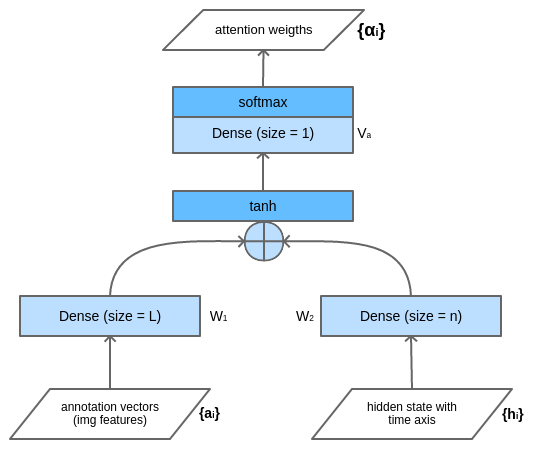
\includegraphics[scale=0.5]{images/ch4/attention-architecture.png}
	\caption{Detailed architecture of the additive soft attention mechanism}
	\label{fig:attention-architecture}
\end{figure}

\section{Data pipelines}

This section describes the data preparation steps needed to train our model over a benchmark dataset such as MS COCO.
Training the proposed model over a big dataset will required

\section{Training}

\section{Inference}



% The visualization of the attention weights clearly demonstrates which regions of the image the model pays attention to so as to output a certain word.
